\documentclass[12pt,letterpaper]{article}

\usepackage[titletoc]{appendix}
\usepackage[compatibility=true]{caption}

\usepackage{fullpage, listings, footnote, graphicx, multicol, enumitem, latexsym, placeins, longtable}
\usepackage{algorithm, algpseudocode}

\usepackage{pgfplotstable}
% recommended:
\usepackage{booktabs}
\usepackage{array}
\usepackage{colortbl}

\usepackage[backend=biber,style=numeric]{biblatex}

\usepackage{hyperref}
\usepackage[noabbrev]{cleveref}

\usepackage{amsmath}

\DeclareLanguageMapping{american}{american-apa}
\addbibresource{Lab5.bib}

\setdescription{leftmargin=\parindent,labelindent=\parindent}
\pdfpxdimen=\dimexpr 1 in/72\relax
\lstdefinestyle{appendixJava}{%
  belowcaptionskip=1\baselineskip,
  breaklines=true,
  xleftmargin=\parindent,
  xrightmargin=\parindent,
  language=Java,
  showstringspaces=false,
  basicstyle=\small,
  numberstyle=\tiny,
  keywordstyle=\bfseries,
  commentstyle=\itshape,
  numbers = left,
  tabsize=4,
}
\lstdefinestyle{log}{%
  belowcaptionskip=1\baselineskip,
  breaklines=true,
  frame=tb,
  xleftmargin=\parindent,
  xrightmargin=\parindent,
  showstringspaces=false,
  basicstyle=\footnotesize\ttfamily,
  tabsize=4,
}

\pgfplotsset{compat=1.8}

\pgfplotstableset{
    begin table=\begin{longtable},
    end table=\end{longtable},
    row sep=\\,
    every head row/.append style={after row=\endhead, before row=\caption{Job queue used to generate the \url{jimweller.com} dataset \cite{jimweller}.}\\},
	alias/Initial burst mode/.initial=0,
	alias/Delay/.initial=1,
	alias/Priority/.initial=2,
}

\author{Hawk Weisman\\CMPSC440: Operating Systems}
\title{Lab 5: Using Simulation to Evaluate Scheduling Algorithms}
\date{Monday, March 10th, 2014}

\begin{document}

	\maketitle
	\tableofcontents
  	\section{Introduction}

  		Scheduling algorithm selection is an extremely important decision in operating system design. Choosing a process scheduler can have significant influence on system performance metrics such as wait time, response time, and turnaround time. However, the workloads which these algorithms must schedule vary sigificantly, they are difficult to study analytically. Simulation, therefore, is a useful tool for investigating the performance of various scheduling algorithms.

  	\section{Methods}

  		\subsection{Simulation \& Metrics}
	  		A CPU simulator implemented by Jim Weller was used to assess various scheduling algorithms. The simulator is available at \url{http://jimweller.com/jim-weller/jim/java_proc_sched/}.

	  		\begin{figure}[H]
				\centerline{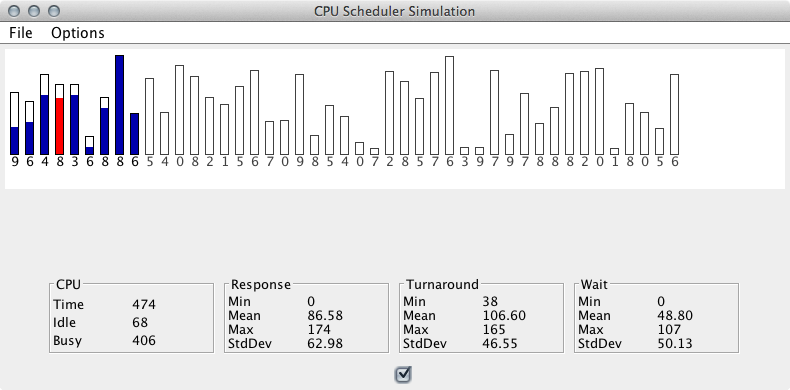
\includegraphics[width=0.80\textwidth]{figures/sim.png}}
				\caption{A screenshot of the CPU simulator implemented by Jim Weller.}
				\label{fig:screenshot}
			\end{figure}

			Seven scheduling algorithms were tested: first come, first serve; preemptive and non-preemptive priority; prioritized and non-prioritized round-robin; and preemptive and non-preemptive shortest job first. 
			\subsubsection{Summary of Scheduling Algorithm}
			\begin{description}[leftmargin=4cm, style=multiline]
					\item[First come, first served]{Also known as \textit{first in, first out}. Probably the simplest scheduling algorithm, this algorithm simply executes jobs in order of their arrival in the ready queue.}
					\item[Shortest job first]{This algorithm schedules jobs in order of length, executing the shortest jobs first.}
						\begin{description}[style=nextline, font=\normalfont\itshape]
							\item[non-preemptive]{In this variant, once a job has begun executing, it will continue executing until it has finished.}
							\item[preemptive]{Unlike the non-preemptive variant, if a job which is shorter than the current job arrives in the ready queue, this algorithm will stop executing the current job and begin executing the shorter job.}
						\end{description}
					\item[Priority]{This algorithm schedules jobs according to priority, executing the highest-priority jobs first.}
						\begin{description}[style=nextline, font=\normalfont\itshape]
							\item[non-preemptive]{In this variant, once a job has begun executing, it will continue executing until it has finished.}
							\item[preemptive]{Unlike the non-preemptive variant, if a job with a higher priority than current job arrives in the ready queue, this algorithm will preempt execution of the current job and begin executing the higher-priority job.}
						\end{description}
					\item[Round robin]{Round robin scheduling assigns each process a \textit{time quantum}, or amount of time over which it may execute, and allows each process in the ready queue to execute for the time quantum in order. If a job is not finished at the end of the time quantum, the scheduler interrupts it and allows the next job to execute. It will then be allowed to resume execution once the scheduler reaches its position in the queue again.}
						\begin{description}[style=nextline, font=\normalfont\itshape]
							\item[non-prioritized]{The non-prioritized round robin variant rotates between all jobs in the ready queue, regardless of priority.}
							\item[prioritized]{The prioritized round robin variant preferrentially rotates between all of the highest priority jobs. If there are no jobs of the highest priority in the ready queue, it will try to alternate between jobs of the next-highest priority level.} 
						\end{description}
				\end{description}

			The CPU simulator recorded the time when each simulated process arrived in the ready queue, when it began execution, and when it finished. This allows for the calculation of the following performance metrics:

				\begin{description}[leftmargin=4.5cm, style=sameline]
					\item[Response Time]{The amount of time between when a job enters the ready queue and when the first response is produced. $T_{response} = T_{first response} - T_{entry}$}
					\item[Wait Time]{The amount of time a job spends in the ready queue before it may begin execution. $T_{wait} = T_{start} - T_{entry}$}
					\item[Turnaround Time]{The amount of time between when a job arrives in the ready queue and when it completes execution. $T_{turnaround} = T_{complete} - T_{entry}$}
				\end{description}

			All of these can be considered lower-is-better metrics, as lower response times, turnaround times, and wait times all indicate a faster system.

			It is also important to note that there is apparently some dispute on the meaning of the term ``turnaround time''. Some sources, such as Andrew Tanenbaum in \textit{Modern Operating Systems}, define turnaround time as ``the statistically average time from the moment that a batch job is submitted until the moment it is completed \cite{tanenbaum2007modern}'', while Jim Weller, who implemented the CPU simulation tool, defines it as ``[t]he total life of the process in the ready queue \cite{jimweller}.'' Since we can assume that Weller's simulation tool calculates turnaround time based on his definition, I have chosen to use that definition in this paper.

			Multiple datasets were used in this study: one provided by Jim Weller for download at \url{http://jimweller.com/jim-weller/jim/java_proc_sched/} (\cref{table:data-jim}) \cite{jimweller}, and five which were generated from random workloads produced using the random workload setting in the CPU simulator tool. \Cref{table:data-rands} shows a summary of the data from all five randomly-generated workloads, while \cref{table:data-rand1,table:data-rand2,table:data-rand3,table:data-rand4,table:data-rand5} in \cref{app:data} show summaries of each individual random workload. Information collected from the randomized workload runs was analyzed both as individual datasets and as one merged dataset. The workload used by Jim Weller to generate the \texttt{jimweller.com} dataset is given in \cref{table:jim-queue} \cite{jimweller}; unfortunately, the simulation tool does not offer a method for saving the job queue from random workloads, so these job queues have not been reprinted.

		\subsection{Data Analysis \& Visualization}
			Data collected from the simulation was analyzed using the IPython interactive computing environment \cite{ipython}, using the Pandas library \cite{ pandas} for statistical analysis. Visualizations were prepared using Matplotlib \cite{matplotlib}. A static copy of the IPython notebook used to analyze and visualize the data may be viewed at \url{http://nbviewer.ipython.org/gist/hawkw/9439505}.

			Box-and-whisker plots were produced to show the distribution of the data collected for each scheduling algorithm. Box-and-whisker plots were chosen to present this data as they allow the distribution of performance observations to be compared across scheduling algorithms in one figure. \Cref{fig:jim_whisker_response,fig:jim_whisker_wait,fig:jim_whisker_turn} show the distributions of response time, wait time, and turnaround time for the \url{jimweller.com} dataset, while \cref{fig:rand_whisker_response,fig:rand_whisker_wait,fig:rand_whisker_turn} show these distributions for the five randomly generated workloads. In these plots, the box encompasses the inter-quartile range with the median marked as a horizontal line. The whiskers extend to 1.5 times the inter-quartile range past the closest quartile, with observations folling outside that range marked as outliers. 

  	\section{Results \& Analysis}

  		\subsection{Data downloaded from \texttt{jimweller.com}}

	  		\Cref{table:data-jim} summarizes the dataset downloaded from \url{http://jimweller.com/jim-weller/jim/java_proc_sched/} \cite{jimweller}.

	  		\begin{table}
	  			\caption{Data from \url{www.jimweller.com}}
		  		\begin{tabular}{l r r r r}
					\textbf{Shortest Job First} & mean & standard deviation & minimum & maximum\\
					\hline
	Wait time &		23.4 &	33.1499622926 & 0 & 147 	 	\\
	Response time &		23.4 &	33.1499622926 &	0 &	147 	\\
	Turnaround time &	54.02 &	48.4555425106 &	3 &	246 	\\
					\\
					\textbf{Shortest Job First (preemptive)} \\
					\hline
	Wait time &		18.24 &	38.6717261058 &	0 &	187 	\\
	Response time &		13.68 &	31.2681563256 &	0 &	147 	\\
	Turnaround time &	48.86 &	56.9677136631 &	3 &	286 	\\
					\\
					\textbf{First Come, First Serve} \\
					\hline
	Wait time &		34.7 &	43.2301977789 &	0 &	156 	\\
	Response time &		34.7 &	43.2301977789 &	0 &	156 	\\
	Turnaround time &	65.32 &	49.252995848 &	3 &	196 	\\
					\\
					\textbf{Round-robin} \\
					\hline
	Wait time &		39.96 &	48.3060907133 &	0 &	197	\\
	Response time &		7.64 &	11.329183554 &	0 &	46 	\\
	Turnaround time &	70.58 &	65.1457105265 &	3 &	296 	\\
					\\
					\textbf{Round-robin (prioritized)} \\
					\hline
	Wait time &		41.6 &	49.9159293212 &	0 &	194 	\\
	Response time &		27.44 &	31.9137337208 &	0 &	108 	\\
	Turnaround time &	72.22 &	60.8411998567 &	3 &	250 	\\
					\\
					\textbf{Priority} \\
					\hline
	Wait time &		28.52 &	57.4387465044 &	0 &	363	\\
	Response time &		28.52 &	57.4387465044 &	0 &	363 	\\
	Turnaround time &	59.14 &	65.0744220105 &	3 &	386 	\\
					\\
					\textbf{Priority (preemptive)} \\
					\hline
	Wait time &		34.34 &	84.741161191 &	0 &	429 	\\
	Response time &		18.2 &	55.246357346 &	0 &	363 	\\
	Turnaround time &	64.96 &	95.8546733342 &	3 &	528 	\\

					\\
				\end{tabular}
				\label{table:data-jim}
			\end{table}

	  	  	\begin{figure}[H]
				\centerline{\includegraphics[width=\textwidth]{figures/weller_whisker_response.pdf}}
				\caption{Box-and-whisker plot of response time (\url{www.jimweller.com} data).}
				\label{fig:jim_whisker_response}
			\end{figure}

	  			In the \url{jimweller.com} dataset (\cref{table:data-jim}), the round-robin algorithm offered the best response time, with a mean response time of 7.64 CPU cycles. As seen in \cref{fig:jim_whisker_response}, the second- and third-best response times were offered by the preemptive shortest-job-first and preemptive priority scheduling algorithms, with mean response times of 13.68 and 18.2 CPU cycles, respectively. 

	  			However, \cref{fig:jim_whisker_response} also illustrates that these algorithms had a much greater number of outliers, with standard deviations of 55.246357346 for preemptive priority and 31.2681563256 for preemptive shortest-job-first. Both of these standard deviations are much higher than round robin's standard deviation of 11.329183554 cycles. The outliers for preemptive priority and preemptive shortest-job-first both had much higher maximum values, as well, with maximum observed response times of 363 and 147 cycles, while round-robin had a maximum observed response time of only 46 cycles. 

	  			Both the preemptive and non-preemptive priority scheduling algorithms produced one outlier with an extremely high response time, 363 CPU cycles. Based on the function of these algorithms, we might guess that this outlier represents a very long job of extremely low priority which entered the ready queue early in the simulation but was not allowed to execute until nearly every other job had finished.

	  			The first-come-first-serve algorithm reliably produced the longest response times, with the exceptions of the outliers described in the previous paragraph. Prioritized round-robin also offered relatively poor performance assessed measured in terms of response time.

			\begin{figure}[H]
				\centerline{\includegraphics[width=\textwidth]{figures/weller_whisker_wait.pdf}}
				\caption{Box-and-whisker plot of wait time (\url{www.jimweller.com} data).}
				\label{fig:jim_whisker_wait}
			\end{figure}

			\Cref{fig:jim_whisker_wait} shows that preemptive shortest-job-first offered the lowest mean wait time, with a mean wait time of 18.24 cycles. Non-preemptive shortest-job-first, non-preemptive priority, and preemptive priority all offered reasonably good mean wait times as well, with mean wait times of 23.4 cycles, 28.52 cycles, and 34.34 cycles, respectively.

			Non-prioritized round-robin, despite having the second-highest mean wait time, offered the lowest standard deviation, 11.329183554 cycles, followed by preemptive shortest-job-first, at 31.2681563256 cycles, and prioritized round-robin, at 31.9137337208 cycles. Round robin had the lowest observed maximum response time, 46 cycles, while both priority algorithms had the highest, 363 cycles.

			\begin{figure}[H]
				\centerline{\includegraphics[width=\textwidth]{figures/weller_whisker_turnaround.pdf}}
				\caption{Box-and-whisker plot of turnaround time (\url{www.jimweller.com} data).}
				\label{fig:jim_whisker_turn}
			\end{figure}

			\Cref{fig:jim_whisker_turn} shows the distribution of turnaround times for each scheduling algorithm in the dataset downloaded from Jim Weller's website. Non-preemptive sortest-job-first offers the lowest mean turnaround time, 48.86 cycles. Preemptive shortest-job-first had the second-lowest observed mean turnaround time, 54.02 cycles, and preemptive priority offered the third shortest, 59.14.

			The first-come-first-served algorithm had  the lowest observed maximum turnaround time, 196 cycles, followed by non-preemptive shortest-job-first at 246 cycles and prioritized round-robin at 250 cycles. Non-preemptive shortest-job-first also had the lowest standard deviation, 48.4555425106 cycles, followed closely by first-come-first-serve at 49.252995848 cycles.

  		\subsection{Randomly-generated workloads}

  			Data from the five randomly-generated workloads is presented in \cref{table:data-rands}. Data from each individual run may be viewed in \cref{table:data-rand1,table:data-rand2,table:data-rand3,table:data-rand4,table:data-rand5,}.

  		 	\begin{table}
	  			\caption{Data from all randomly-generated workloads.}
		  		\begin{tabular}{l r r r r}
					\textbf{Shortest Job First} & mean & standard deviation & minimum & maximum\\
					\hline
Wait time &		280.952 &	511.560723371 &	0 &	2399 	\\
Response time &		280.952 &	511.560723371 &	0 &	2399 	\\
Turnaround time &	331.844 &	530.611854055 &	8 &	2492 	\\
					\\
					\textbf{Shortest Job First (preemptive)} \\
					\hline
Wait time &		273.552 &	519.453604565 &	0 &	2399 	\\
Response time &		263.108 &	518.828835297 &	0 &	2399 	\\
Turnaround time &	324.444 &	539.145641607 &	1 &	2492 	\\
					\\
					\textbf{First Come, First Serve} \\
					\hline
Wait time &		470.98 &	320.855836163 &	0 &	1140 	\\
Response time &		470.98 &	320.855836163 &	0 &	1140 	\\
Turnaround time &	521.872 &	321.653887923 &	8 &	1169 	\\
					\\
					\textbf{Round-robin} \\
					\hline
Wait time &		684.1 &	543.761787918 &	0 &	1879 	\\
Response time &		66.312 &	65.0040510738 &	0 &	303 	\\
Turnaround time &	734.992 &	565.47069945 &	1 &	1974 	\\
					\\
					\textbf{Round-robin (prioritized)} \\
					\hline
Wait time &		630.292 &	637.714568389 &	0 &	2459 	\\
Response time &		231.34 &	188.820783814 &	0 &	915 	\\
Turnaround time &	681.184 &	652.677389025 &	8 &	2540 	\\
					\\
					\textbf{Priority} \\
					\hline
Wait time &		462.692 &	591.043366544 &	0 &	2376 	\\
Response time &		462.692 &	591.043366544 &	0 &	2376 	\\
Turnaround time &	513.584 &	592.189668049 &	8 &	2457 	\\
					\\
					\textbf{Priority (preemptive)} \\
					\hline
Wait time &		486.304 &	614.187029808 &	0 &	2468 	\\
Response time &		430.136 &	601.849919418 &	0 &	2376 	\\
Turnaround time &	537.196 &	616.72793806 &	1 &	2560 	\\
					\\
				\end{tabular}
				\label{table:data-rands}
			\end{table}

			\begin{figure}[H]
				\centerline{\includegraphics[width=\textwidth]{figures/rand_whisker_response.pdf}}
				\caption{Box-and-whisker plot of response time across five randomly-generated workloads.}
				\label{fig:rand_whisker_response}
			\end{figure}

			\Cref{fig:rand_whisker_response} shows box-and-whisker plots of response time for each algorithm across the five randomly-generated workloads. As seen in this figure, non-prioritized round-robin had the lowest observed mean response time, 66.312 cycles, followed by prioritized round-robin (231.34 cycles) and preemptive shortest-job-first (263.108 cycles). Non-prioritized round-robin also had the lowest observed standard deviation, 65.0040510738 cycles.

			Despite very low mean response times, both shortest-job-first algorithms had very a high maximum observed response time, 2399 cycles, the highest observed in the dataset. Due to the number of high outliers, which can be observed in \cref{fig:rand_whisker_response}, they also had high standard deviations, with non-preemptive shortest-job-first having a standard deviation of 511.560723371 cycles, and preemptive shortest-job-first having a standard deviation of 518.828835297 cycles.

			\begin{figure}[H]
				\centerline{\includegraphics[width=\textwidth]{figures/rand_whisker_wait.pdf}}
				\caption{Box-and-whisker plot of wait time across five randomly-generated workloads.}
				\label{fig:rand_whisker_wait}
			\end{figure}

			Across the five randomly-generated workloads, preemptive and non-preemptive shortest-job-first also had the lowest and second-lowest observed mean wait times (273.552 and 280.952 cycles), as shown in \cref{fig:rand_whisker_wait}. The standard deviations for preemptive and non-preemptive shortest-job-first were 519.453604565 and 511.560723371 cycles, respectively. The maximum observed wait times for both shortest-job-first algoritms were 2399 cycles. Preemptive priority had the third-lowest observed mean wait time, 462.692 cycles. 

			First-come-first-serve had a much higher mean wait time, 470.98 cycles, but it also had the lowest observed standard deviation, 320.855836163 cycles, and the lowest observed maximum wait time, 1140 cycles. Prioritized round-robin is perhaps the least effective algorithm when judged in terms of wait time alone, with a mean wait time of 630.292 cycles and a standard deviation of 637.714568389.

			\begin{figure}[H]
				\centerline{\includegraphics[width=\textwidth]{figures/rand_whisker_turnaround.pdf}}
				\caption{Box-and-whisker plot of turnaround time across five randomly-generated workloads.}
				\label{fig:rand_whisker_turn}
			\end{figure}

			\Cref{fig:rand_whisker_turn} shows the distribution of turnaround times across the five randomly-generated workloads. Preemptive and non-preemptive shortest-job-first had the lowest and second-lowest observed mean turnaround times, 324.444 cycles for the preemptive algorithm and 331.844 cycles for the algorithm without preemption. The standard deviations for these two algorithms were both mid-range, with the algorithm without preemption having a slightly lower standard deviation of 530.611854055 cycles, and the algorithm with preemption having a slightly higher standard deviation of 539.145641607 cycles.

			First-come-first-serve had the lowest maximum observed wait time, 1169 cycles, followed by non-prioritized round-robin, which had a maximum observed wait time of 1974 cycles. Preemptive priority had the highest observed maximum response time, 2560 cycles, followed by prioritized round-robin, with a maximum observed response time of 2540 cycles. Prioritized round-robin also had the highest standard deviation, 652.677389025 cycles, and preemptive priority had the second-highest standard deviation, 616.72793806 cycles. Non-prioritized round-robin had the highest observed mean turnaround time, 734.992 cycles.

  	\section{Discussion}

  		\subsection{Assessment of Scheduling Algorithms}

  			In order to assess which of the scheduling algorithms under study is the best suited for a modern operating system, we must determine which of the characteristics measured are the most important for modern interactive systems. We must also determine what precisely is meant by the phrase ``modern operating systems''. In this case, we will consider ``modern operating systems'' to refer to interactive, single-user operating systems with graphical user interfaces, in contrast to command-line only systems, multi-user timesharing systems, and batch systems.

  			According to Tanenbaum in \textit{Modern Operating Systems}, 3rd Ed., in interactive systems, the most important goal is to minimize response time \cite{tanenbaum2007modern}. This is because on most modern operating systems, many processes are typically running in the background non-interactively, providing services to other programs in the system. These processes might include jobs carrying out actions such as fetching new emails from the network, saving backups to an external drive, and performing other services which, while useful, are not immediately apparent to the user. Tanenbaum points out that in an interactive system, user processes that create immediately apparent responses should take priority over this background work, as ``having all interactive requests go first will be perceived as good service \cite{tanenbaum2007modern}'' --- the user may not be aware that the execution of their commands is delayed due to a background process, but they will certainly notice that theirlv computer is acting sluggish. While characteristics such as turnaround time and wait time are certainly important, designers of interactive single-user systems might find it wise to preferentially optimize for response time, based on Tanenbaum's obervation.

  			Tanenbaum also makes the related observation that users frequently have expectations of how long certain tasks take, and that while these expectations may not always be correct, users are much more willing to accept tasks which they perceive as complex taking long amounts of time to complete \cite{tanenbaum2007modern}. Users are willing to wait for complex tasks, such as applying a filter to an image or rendering a 3D model, but if tasks they consider to be simple, such as closing a window, launching a program, or opening a file, take a long amount of time, they will quickly become irritated. Therefore, it is important to schedule tasks in a way that conforms to user expectations. The standard deviations of scheduling algorithms observed in the study provide a method to assess the predictability of scheduling performance - if an algorithm has a very low mean response time, but a very high standard deviation and a maximum observed response time which is much higher than the mean, that implies that it generally offers good performance, but there are some situations --- pathological cases --- in which response times will be significantly longer.

  			Based on these observations, we now have a picture of what characteristics are ideal for a modern operating system. \Cref{table:data-jim,table:data-rands} indicate that in both the \url{jimweller.com} dataset and in the dataset from the five randomly-generated workloads, the non-prioritized round-robin scheduling algorithm offered the lowest mean response time. While round-robin provides middle-of-the-road mean wait times and turnaround times, those characteristics are less important to the designers of interactive systems. It also offers the lowest standard deviation of response times, indicating that response times will be relatively predictable and therefore conform to user expectations. 

  			Tanenbaum also points out that round-robin is very easy to implement, since all the scheduler must do is maintain a queue of processes, allow the process at the head of the queue to execute for its time quantum, and then move it to the tail of the queue if it is not yet finished executing \cite{tanenbaum2007modern}. Determining the length of the time quantum is the only difficult problem involved with implementing round-robin scheduling. 

  			If preferential execution of high-priority processes is important, prioritized round-robin may be implemented through the use of multiple queues corresponding to each priority level. While the mean response time for the prioritized round-robin algorithm is lower than both the non-prioritized round-robin and the preemptive priority algorithm in the \url{jimweller.com} dataset (\cref{table:data-jim})), this is not true in the dataset observed from the five randomly-generated workloads (\cref{table:data-rands}), where prioritized round-robin offered a lower observed mean response time than both preemptive and non-preemptive priority-based scheduling. Furthermore, in both datasets, prioritized round-robin had much lower maximum response times and standard deviations than the priority-based algorithms, implying much more predictable performance. 

  		\subsection{Difficulties \& Opportunities for Further Study}

  			A major flaw in this study is that the metrics collected (response time, wait time, and turnaround time) are all measurements of \textit{performance}. While performance is a major concern in the implementation of schedulers, operating systems designers are also interested in other characteristics, such as \textit{fairness}, ensuring that equal CPU time is distributed to each process, and the related idea of \textit{proportionality}, like fairness but ensuring that CPU time is distributed to each process according to its priority and workload; \textit{throughput}, the total number of processes that complete execution over a given time interval, and \textit{utilization}, ensuring that the most efficient possible use is made of the CPU and other system resources. A more comprehensive study of scheduling algorithms might record information on these qualities as well.

  			It's important to note that the simulation recorded response times, wait times, and turnaround times for all jobs as a group, and did not track these metrics independantly for jobs of each priority. If our goal is to maximize these metrics for higher priority jobs, rather than for all jobs, we might find that algorithms such as priority and preemptive priority, which offered relatively poor overall performance, might offer significantly better performance for high-priority jobs when compared to more egalitarian algorithms such as shortest-job-first.

  			Another issue is that of \textit{representativeness}. Since  simulation-based studies by definition do not involve data collected from real-world machines, it is important to ensure that the inputs to the simulation are representative of the actual conditions under which the algorithms under study must function. In the case of scheduling algorithms, this means that the characteristics of the workload, such as the burst time, or amount of CPU time each process requires to execute; the delay in the rate at which new processes enter the ready queue; and the distribution of priorities assigned to processes entering the ready queue, must all be made as close as possible to the characteristics of the workloads on real-world machines. Otherwise, the results of the simulation will not be very valuable for making decisions in the real world.

  			More representative simulation inputs might be prepared by conducting observations of the workload characteristics of a wide range of actual computers, analyzing those observations, and constructing a workload or set of workloads based on the patterns found in these observations. Those workloads could then be used as input to simulations with the understanding that they represent with some accuracy the conditions under which scheduling algorithms will actually operate.

	\begin{appendices}

		\section{Data}
			\label[appendix]{app:data}

			\subsection{Random Workload I}
			\begin{table}[H]
	  			\caption{Data from the first random workload.}
		  		\begin{tabular}{l r r r r}
					\textbf{Shortest Job First} & mean & standard deviation & minimum & maximum\\
					\hline
					Wait time &		343.42 &	551.749112913 &	0 &	2067 	\\
					Response time &		343.42 &	551.749112913 &	0 &	2067 	\\
					Turnaround time &	394.66 &	572.012328888 &	24 &	2162 	\\
					\\
					\textbf{Shortest Job First (preemptive)} \\
					\hline
					Wait time &		335.64 &	557.678680245 &	0 &	2067 	\\
					Response time &		326.82 &	560.773347797 &	0 &	2067 	\\
					Turnaround time &	386.88 &	578.559785675 &	3 &	2162 	\\
					\\
					\textbf{First Come, First Serve} \\
					\hline
					Wait time &		583.64 &	272.881421867 &	0 &	993  	\\
					Response time &		583.64 &	272.881421867 &	0 &	993 	\\
					Turnaround time &	634.88 &	269.476428654 &	65 &	999 	\\
					\\
					\textbf{Round-robin} \\
					\hline
					Wait time &		860.24 &	517.426074333 &	1 &	1819  	\\
					Response time &		82.94 &	71.8894734993 &	0 &	298 	\\
					Turnaround time &	911.48 &	541.01261501 &	11 &	1914 	\\
					\\
					\textbf{Round-robin (prioritized)} \\
					\hline
					Wait time &		830.4 &	670.613778564 &	45 &	2042  	\\
					Response time &		287.26 &	112.772658034 &	0 &	466 	\\
					Turnaround time &	881.64 &	686.207658366 &	80 &	2137 	\\
					\\
					\textbf{Priority} \\
					\hline
					Wait time &		584.94 &	630.010203409 &	0 &	2365 	\\
					Response time &		584.94 &	630.010203409 &	0 &	2365 	\\
					Turnaround time &	636.18 &	628.436876385 &	18 &	2405 	\\
					\\
					\textbf{Priority (preemptive)} \\
					\hline
					Wait time &		600.24 &	635.131909449 &	0 & 2365 	\\
					Response time &		562.94 &	647.064831682 &	0 &	2365 	\\
					Turnaround time &	651.48 &	634.430145564 &	15 &	2405 	\\
					\\
				\end{tabular}
				\label{table:data-rand1}
			\end{table}

			\subsection{Random Workload II}

				\begin{table}[H]
		  			\caption{Data from the second random workload.}
			  		\begin{tabular}{l r r r r}
						\textbf{Shortest Job First} & mean & standard deviation & minimum & maximum\\
						\hline
	Wait time &		426.02 &	661.628944046 &	0 &	2399	\\
	Response time &		426.02 &	661.628944046 &	0 &	2399 	\\
	Turnaround time &	482.78 &	681.05621765 &	8 &	2492 	\\
						\\
						\textbf{Shortest Job First (preemptive)} \\
						\hline
	Wait time &		417.32 &	676.881716107 &	0 &	2399	\\
	Response time &		400.6 &	672.674007228 &	0 &	2399 	\\
	Turnaround time &	474.08 &	696.785787456 &	1 &	2492 	\\
						\\
						\textbf{First Come, First Serve} \\
						\hline
	Wait time &		677.76 &	329.807068451 &	0 &	1070 	\\
	Response time &		677.76 &	329.807068451 &	0 &	1070 	\\
	Turnaround time &	734.52 &	326.00596559 &	8 &	1155 	\\
						\\
						\textbf{Round-robin} \\
						\hline
	Wait time &		1013.34 &	562.567564298 &	0 &	1879	\\
	Response time &		96.08 &	79.6765561505 &	0 &	303 	\\
	Turnaround time &	1070.1 &	588.339706292 &	8 &	1974 	\\
						\\
						\textbf{Round-robin (prioritized)} \\
						\hline
	Wait time &		912.66 &	666.017885946 &	0 &	2459 	\\
	Response time &		386.0 &	181.003093896 &	0 &	914 	\\
	Turnaround time &	969.42 &	680.328129361 &	8 &	2540 	\\
						\\
						\textbf{Priority} \\
						\hline
	Wait time &		691.06 &	691.35957099 &	0 &	2376 	\\
	Response time &		691.06 &	691.35957099 &	0 &	2376 	\\
	Turnaround time &	747.82 &	688.458733404 &	8 &	2457 	\\

						\\
						\textbf{Priority (preemptive)} \\
						\hline
	Wait time &		698.86 &	689.455901708 &	0 &	2376 	\\
	Response time &		683.2 &	698.788379984 &	0 &	2376 	\\
	Turnaround time &	755.62 &	686.830281511 &	8 &	2457 	\\
						\\
					\end{tabular}
					\label{table:data-rand2}
				\end{table}

			\subsection{Random Workload III}

			\begin{table}[H]
	  			\caption{Data from the third random workload.}
		  		\begin{tabular}{l r r r r}
					\textbf{Shortest Job First} & mean & standard deviation & minimum & maximum\\
					\hline
Wait time &			96.92 &	182.14102668 &	0 &	946 	\\
Response time &		96.92 &	182.14102668 &	0 &	946 	\\
Turnaround time &	140.76 &	200.524568071 &	12 &	1045 	\\
					\\
					\textbf{Shortest Job First (preemptive)} \\
					\hline
Wait time &			89.06 &	192.054097587 &	0 &	946 	\\
Response time &		80.68 &	187.227288609 &	0 &	946 	\\
Turnaround time &	132.9 &	211.815603769 &	1 &	1045 	\\
					\\
					\textbf{First Come, First Serve} \\
					\hline
Wait time &			182.52 &	141.884211948 &	0 &	454 	\\
Response time &		182.52 &	141.884211948 &	0 &	454 	\\
Turnaround time &	226.36 &	140.215799395 &	16 & 498 	\\
					\\
					\textbf{Round-robin} \\
					\hline
Wait time &			226.32 &	216.027724147 &	0 &	785 	\\
Response time &		27.12 &	24.9556727018 &	0 &	87 	\\
Turnaround time &	270.16 &	237.121349524 &	1 &	884 	\\
					\\
					\textbf{Round-robin (prioritized)} \\
					\hline
Wait time &			252.22 &	273.411432826 &	0 &	1197 	\\
Response time &		99.72 &	85.1964881905 &	0 &	368 	\\
Turnaround time &	296.06 &	288.366184564 &	16 &	1281 	\\
					\\
					\textbf{Priority} \\
					\hline
Wait time &			212.92 &	327.833118522 &	0 &	1475	\\
Response time &		212.92 &	327.833118522 &	0 &	1475 	\\
Turnaround time &	256.76 &	323.014585429 &	15 &	1513 	\\
					\\
					\textbf{Priority (preemptive)} \\
					\hline
Wait time &			271.04 &	411.399317452 &	0 &	1885 	\\
Response time &		182.54 &	335.130554262 &	0 &	1475 	\\
Turnaround time &	314.88 &	409.753225247 &	1 &	1910 	\\
					\\
				\end{tabular}
	 			\label{table:data-rand3}
			\end{table}

			\subsection{Random Workload IV}
			\begin{table}[H]
	  			\caption{Data from the fourth random workload.}
		  		\begin{tabular}{l r r r r}
					\textbf{Shortest Job First} & mean & standard deviation & minimum & maximum\\
					\hline
Wait time &			323.98 &	548.49399231 &	0 &	2198 	\\
Response time &		323.98 &	548.49399231 &	0 &	2198 	\\
Turnaround time &	378.54 &	568.75120079 &	10 &	2297 	\\
					\\
					\textbf{Shortest Job First (preemptive)} \\
					\hline
Wait time &			318.86 &	552.158673209 &	0 &	2198 	\\
Response time &		313.46 &	553.946286566 &	0 &	2198 	\\
Turnaround time &	373.42 &	572.948936294 &	4 &	2297 	\\
					\\
					\textbf{First Come, First Serve} \\
					\hline
Wait time &			528.64 &	339.63437753 &	0 &	1140 	\\
Response time &		528.64 &	339.63437753 &	0 &	1140 	\\
Turnaround time &	583.2 &	340.075403403 &	75 &	1169 	\\
					\\
					\textbf{Round-robin} \\
					\hline
					Wait time &		777.76 &	541.151533676 &	28 &	1699 	\\
Response time &		64.1 &	61.2732404888 &	0 &	237 	\\
Turnaround time &	832.32 &	565.286456233 &	37 &	1794 	\\
					\\
					\textbf{Round-robin (prioritized)} \\
					\hline
					Wait time &		664.16 &	622.604797926 &	9 &	2253	\\
Response time &		287.6 &	238.845054376 &	0 &	915 	\\
Turnaround time &	718.72 &	637.174200357 &	51 &	2336 	\\
					\\
					\textbf{Priority} \\
					\hline
					Wait time &		494.34 &	615.176449809 &	0 &	2168  	\\
Response time &		494.34 &	615.176449809 &	0 &	2168 	\\
Turnaround time &	548.9 &	618.453433979 &	12 &	2251 	\\
					\\
					\textbf{Priority (preemptive)} \\
					\hline
					Wait time &		532.82 &	672.008770478 &	0 &	2468 	\\
Response time &		427.6 &	615.420376653 &	0 &	2168 	\\
Turnaround time &	587.38 &	678.312019354 &	9 &	2560 	\\
					\\
				\end{tabular}
	 			\label{table:data-rand4}
			\end{table}

			\subsection{Random Workload V}
			\begin{table}[H]
	  			\caption{Data from the fifth random workload.}
		  		\begin{tabular}{l r r r r}
					\textbf{Shortest Job First} & mean & standard deviation & minimum & maximum\\
					\hline
Wait time &		214.42 &	408.874361632 &	0 &	1518	\\
Response time &		214.42 &	408.874361632 &	0 &	1518 	\\
Turnaround time &	262.48 &	427.537705472 &	9 &	1616 	\\
					\\
					\textbf{Shortest Job First (preemptive)} \\
					\hline
					Wait time &		206.88 &	416.127943787 &	0 &	1518 	\\
Response time &		193.98 &	416.523636304 &	0 &	1518 	\\
Turnaround time &	254.94 &	435.665211372 &	3 &	1616 	\\
					\\
					\textbf{First Come, First Serve} \\
					\hline
					Wait time &		382.34 &	214.89900977 &	0 &	665 	\\
Response time &		382.34 &	214.89900977 &	0 &	665 	\\
Turnaround time &	430.4 &	213.661788816 &	14 &	705 	\\
					\\
					\textbf{Round-robin} \\
					\hline
					Wait time &		542.84 &	420.649562463 &	0 &	1464  	\\
Response time &		61.32 &	50.0553453689 &	0 &	177 	\\
Turnaround time &	590.9 &	440.933747858 &	14 &	1559 	\\
					\\
					\textbf{Round-robin (prioritized)} \\
					\hline
					Wait time &		492.02 &	628.272727086 &	0 &	1842 	\\
Response time &		96.12 &	51.5851296402 &	0 &	198 	\\
Turnaround time &	540.08 &	643.555089794 &	14 &	1931 	\\
					\\
					\textbf{Priority} \\
					\hline
					Wait time &		330.2 &	487.663285475 &	0 &	1706 	\\
Response time &		330.2 &	487.663285475 &	0 &	1706 	\\
Turnaround time &	378.26 &	492.236683314 &	14 &	1798 	\\
					\\
					\textbf{Priority (preemptive)} \\
					\hline
					Wait time &		328.56 &	504.969708398 &	0 &	1706	\\
Response time &		294.4 &	501.648323031 &	0 &	1706 	\\
Turnaround time &	376.62 &	510.908050044 &	4 &	1798 	\\
					\\
				\end{tabular}
	 			\label{table:data-rand5}
			\end{table}

	\pagebreak
	\section{Job Workloads}

		\pgfplotstabletypeset[
			col sep=comma,
			header=false,   
			columns={Initial burst mode,Delay,Priority},
			]{data/jobQueue.csv}		    
			\label{table:jim-queue}

	\end{appendices}

	\clearpage
	\addcontentsline{toc}{section}{References}
	\printbibliography
\end{document}